\label{chapter:conceitos}
O principal objetivo desse capítulo é apresentar conceitos necessários para o entendimento deste trabalho, de forma clara e direta. Os assuntos abordados neste capítulo são: Comunicação sem fio, Localização e Algoritmos de localização RFID.
\section{Sistemas Embarcados}
    \par
    Segundo \citeauthor{rodrigo2016} sistemas embarcados estão presente em quase todos os ambientes, tais sistemas possuem uma única função específica e que não pode ser alterada. Eles são controlados por microprocessadores ou microcontroladores de forma que possuem muitas restrições em relação a recursos computacionais.

    \par
    Atualmente é possível encontrar sistemas embarcados em diversos dispositivos, por exemplo: televisores, micro-ondas, sistemas de gerenciamento de aviação, esteiras, etc. Os dispositivos que fazem uso de eletricidade para seu funcionamento, basicamente possuem um sistema embarcado para articular o seu funcionamento \cite{rodrigo2016}.
    
    \par
    Na \autoref{fig:sistemas embarcados} estão alguns dos aparelhos em que é possível se encontrar sistemas embarcado. É possível notar que aparelhos antigos já utilizavam tal sistemas e com o passar dos anos cada vez mais estão sendo introduzidos nos eletrônicos.
    \begin{figure}[h!]
              \caption{\label{fig:sistemas embarcados}{Sistemas Embarcados.}}
              \centering
              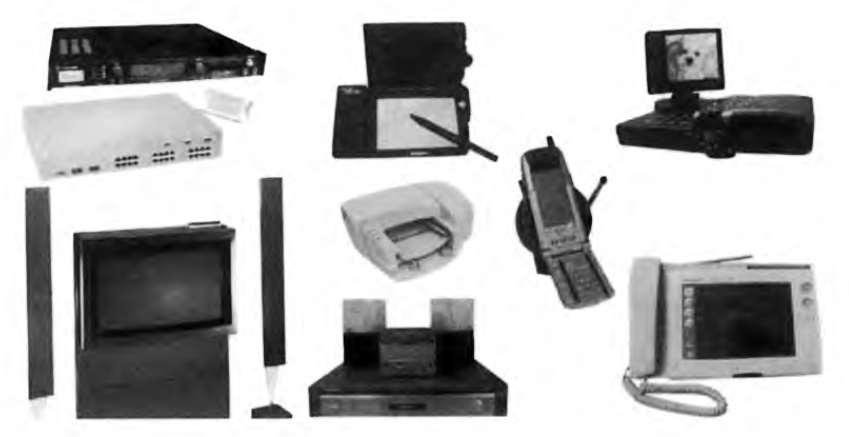
\includegraphics[width=0.5\textwidth]{Figuras/systems_embedded.PNG}
              \legend{Fonte: \cite{Li:2003:RCE:829584}}
            \end{figure}
    \par
    Uma definição geral para sistemas embarcados: são sistemas que realizam uma função dedica e possuem a integração de hardware e software fortemente acoplados, geralmente são uma parte específica de um sistema maior \cite{Li:2003:RCE:829584}.
    % microcontroladores e microprocessadores
    
    % Sistemas de tempo real e tolerancia a falha
    

    \subsection{IoT}
    \par
    A possibilidade de comunicação entre objetos de uso cotidiano do ambiente real com a internet referência o termo IoT, quando um objeto está conectado a rede de computadores e passa a transmitir informações de seu funcionamento ou estado, tal objeto passa a ser denominado de objeto inteligente \cite{iot2016}.
    \par
    De acordo com \citeauthor{iot2017}, o conceito de IoT não é novo, pois desde os passos iniciais da internet ja se pensava em formas de traçar a comunicação entre objetos do dia a dia com a internet. Com os avanços de sistemas embarcados o desenvolvimento de uma infinidades de padrões e protocolos para a integração de WSN tornaram IoT uma realidade.
    \begin{figure}[H]
              \caption{\label{fig:iot}{Internet of Things.}}
              \centering
              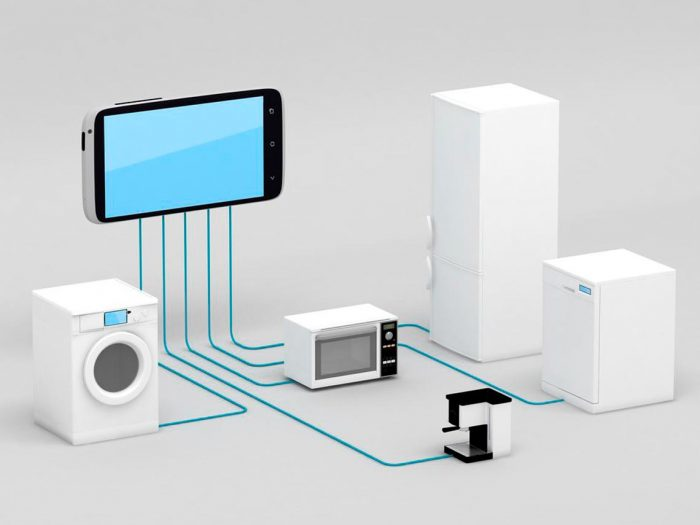
\includegraphics[width=0.5\textwidth]{Figuras/iot.png}
              \legend{Fonte: \cite{imgIot}}
        \end{figure}
    \par
    A \autoref{fig:iot} representa bem o cenário que IoT proporciona, na imagem é possível notar que todos os objetos estão conectado por uma espécie de cabo azul, mas isso é so uma representação, essa conexão também pode ser através de conectividade sem fio. Ainda sobre a imagem, o \textit{smartphone} tem um papel interesante, pois ele está sendo o encarregado de mostrar as informações enviadas pelos objetos para o usuário.
    % relação de iot com sistemas embarcados
    
\section{Comunicação Sem Fio}
    \par
    A medida que os elétrons se movimentam ondas eletromagnéticas são criada no espaço, essas ondas são medidas de acordo com suas oscilações e chamadas de frequência (Hertz), o comprimento dessa onda é medido pela distância de dois pontos máximos ou dois pontos minímos seguidos \cite{tenenbaum2002}.
    \par
    Segundo \citeauthor{tenenbaum2002} ao colocar uma antena em um circuito elétrico apropriado pode-se  transmistir e receber ondas eletromagnéticas, a comunição sem fio é baseada nisso.
    
    \subsection{Transmissão por rádio}
        % o que é 
        
        \par
        A transmissão de dados por rádio pode acontecer de duas maneiras: não-direcional e direcional  \cite{torres2001}.
        
        \begin{itemize}
        \item{Não-Direcional: }
        Quando a transmissão é feita pela forma não-direcional, a frequencias são emitidads em todas as direções e qualquer antena localizada na região de alcance das ondas de rádio podem captar os dados \cite{torres2001}, isso pode ser visto na \autoref{fig:nao_direciona}.
            \begin{figure}[H]
              \caption{\label{fig:nao_direciona}{Transmissão não-direcional.}}
              \centering
              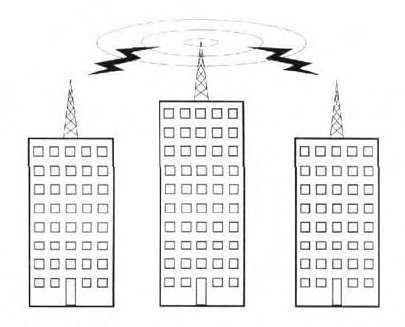
\includegraphics[width=0.5\textwidth]{Figuras/transmissao_radio_nao_direcional.PNG}
              \legend{Fonte: \cite{torres2001}}
            \end{figure}
        \par
        A  \autoref{fig:nao_direciona} mostra que as ondas de radio são emitidas em todas as direções e que qualquer antena/recepetor que estiver no alcance pode receber os dados do emissor.
        
        \item{Direcional: }
        A transmissão no sistema direcional necessita que os aparelhos transmissores e receptores estejam apontando um na direção do outro para que haja comunicação, sem contar que não pode ter obstaculos entre eles senão dificulta a transmissão \cite{torres2001}. A \autoref{fig:direcional} exemplifica o funcionamento dessa forma de transmissão.

        \begin{figure}[H]
              \caption{\label{fig:direcional}{Transmissão direcional.}}
              \centering
              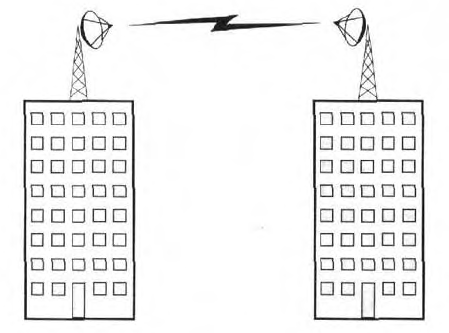
\includegraphics[width=0.5\textwidth]{Figuras/transmissao_radio_direcional.PNG}
              \legend{Fonte: \cite{torres2001}}
        \end{figure}
        \par
        De outro modo a \autoref{fig:direcional} mostra que o primeiro transmissor dever estar direcionado para a direcção do segundo trasmissor, e assim dever acontecer com o segundo transmissor também.
        \end{itemize}    
\section{Localização}
\par
Segundo \citeauthor{rfid2009review}, as informações situacionais de pessoas ou objetos têm um papel muito importante nas aplicações, dessa forma é possível saber a posição dos objetos ou pessoas para assim fazer um monitoramento ou utilizar para várias outras aplicações. Essas informações podem ser obtida através de sistemas de posicionamento, que podem ser classificados dependendo do ambiente, podendo ser destinada a ambientes internos ou externo. Esta seção aborda alguns dos tipos de sistemas de localização.
    \subsection{GPS}
    \par
    GPS é um sistema de posicionamento global implementado pelo programa NAVSTAR \textit{(Navigation System Timing and Ranging)}, iniciado no ano de 1973. Era mantido pela divisão de sistema espacial dos Estados Unidos e era destinado apenas para uso militar \cite{gpsEduardo2005}.
    \par
   O principal objetivo do uso de GPS é determinar as coordenadas espaciais de pontos referentes a um sistema mundial, para isso o sistema faz uso de distâncias entre quatros satélites, a posição do receptor é calculada a partir dos sinais recebido pelos satélites \cite{gpsEduardo2005}.

   \begin{figure}[H]
              \caption{\label{fig:satelites}{Constelação de Satélites.}}
              \centering
              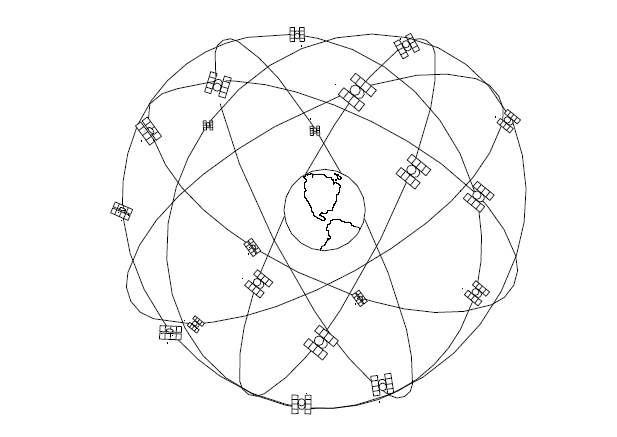
\includegraphics[width=0.5\textwidth]{Figuras/gps_satelites.PNG}
              \legend{Fonte: \cite{gpsEduardo2005}}
        \end{figure}
        \par
        A  \autoref{fig:satelites} mostra a movimentação dos satélites em torno da Terra para assim enviar sinais para os receptores que por sus vez interpretam esses sinais resultando em seu posicionamento na Terra.
 
    \subsection{WLAN\label{subsection:wlan}}
    \par
    A localização em ambientes indoor utilizando WLANs pode ser feita com a RSSI, \textit{Angle of Arrival} (AOA), ou \textit{Time Difference of Arrival} (TDOA) \cite{wifiFernandes}. Os dispositivos devem possuir conectividade sem fio para que seja possível saber seu posicionamento no ambiente. A função que permite a utilização de RSSI está disponível em todas as interfaces 802.11 \cite{Wlan2012}.
    
    \par
    Entre as inúmeras maneiras de localizar dispositivos em ambientes fechados utilizando WLANs, algumas são: 
    \begin{itemize}
        \item {Triangulação}
        \par
        Essa forma de localizar faz uso de AOA, que seria computação dos ângulos a múltiplos ponto de acesso, o resultado disso é uma interceptação que resulta na provável localização, isso pode ser visto na \autoref{fig:triangulacao} \cite{wifiFernandes}. 
           \begin{figure}[H]
              \caption{\label{fig:triangulacao}{Triangulação.}}
              \centering
              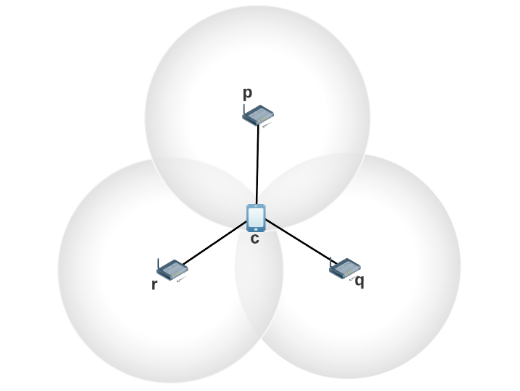
\includegraphics[width=0.5\textwidth]{Figuras/triangulacao.PNG}
              \legend{Fonte: \cite{wifiFernandes}}
        \end{figure}
        \item {Trilateração: }
        \par 
       Utilizando propriedades geométricas essa técnica faz cálculos entre múltiplos pontos de acesso para assim obter a posição do dispositivo \cite{wifiFernandes}.
        \begin{figure}[H]
              \caption{\label{fig:trilateracao}{Trilateração.}}
              \centering
              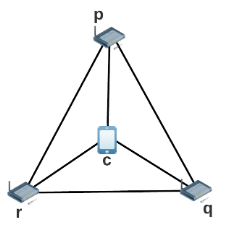
\includegraphics[width=0.5\textwidth]{Figuras/trilateracao.PNG}
              \legend{Fonte: \cite{wifiFernandes}}
        \end{figure}
       \par
        Na \autoref{fig:trilateracao} é mostrado que há uma a comunicação entre os pontos de acesso para assim poder efetuar os cálculos, esses cálculos são uma forma de saber a TDOA para assim estimar a posição do objeto \cite{wifiFernandes}.
        
        \item {Reconhecimento de padrões }
        \par
        O RSS é o principal requisito dessa técnica, em que é feita medições prévias para fazer uma comparação com os dados do banco de dados. Inicialmente é necessário uma fase em que é feita a calibração para se obter o mapa de assinatura \cite{wifiFernandes}.
        
        \par
        O mapa de assinatura é basicamente dados do banco que representam a coleção das medidas de RSSI em diferentes locais para todos os pontos de acesso no ambiente \cite{wifiFernandes}. Na \autoref{fig:fingerprinting} é mostrado seu funcionamento, onde cada ponto de acesso se comunica com o servidor para assim fazer uma comparação com os dados do mapa de assinatura.
         \begin{figure}[H]
              \caption{\label{fig:fingerprinting}{Reconhecimento de padrões.}}
              \centering
              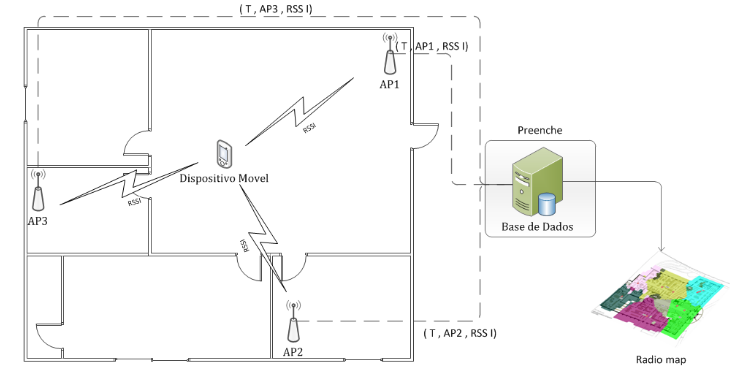
\includegraphics[width=0.9\textwidth]{Figuras/fingerprinting.PNG}
              \legend{Fonte: \cite{wifiFernandes}}
        \end{figure}
    \end{itemize}

    \subsection{RFID}
    \par
    Nessa subseção estaremos mostrando a técnica de localização com RFID utilizada no sistema \textit{LocAlizatioD iDentification based on dynaMic Active Rfid Calibration} (LANDMARC) proposto por \citeauthor{landmarc}, visto que esse sistema é citado na grande maioria das fontes que retratam a utilização de RFID para localizar objetos em ambientes fechados.
    
    \par
    O LANDMARC faz uso de tags RFID ativas para determinar o local das tags que serão localizadas, essas tags ativas são colocadas em pontos já conhecidos pelo sistema e servem como pontos de referência e assim diminuir o número de leitores e ter uma melhor precisão no ambiente \cite{RFIDapplicationsTechniques}.
    
    \par
    Através das tags ativas é possível se obter informações com relação a intensidade do sinal, essa informação é utilizada para calibrar a distância para as tags de rastreio por meio de uma soma com o peso atribuído as tags de referências mais próximas, é importante resaltar que a precisão dos resultados depende da forma que as tags de referência são posicionadas \cite{RFIDapplicationsTechniques}.
    
    \begin{figure}[H]
              \caption{\label{fig:landmarc2a}{LANDMARC.}}
              \centering
              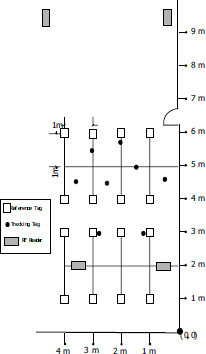
\includegraphics[width=0.4\textwidth]{Figuras/landmarc2a.png}
              \legend{Fonte: \cite{landmarc}}
        \end{figure}
    \par
    Na \autoref{fig:landmarc2a} mostra a aplicação sendo utilizada em um ambiente real por \citeauthor{landmarc}, em que os retangulos cinzas são leitores RFID, os retangulos brancos são tags de refências e os pontos pretos são tags a serem localizadas, e dessa forma o sistema calcula as coordenadas dos objetos.
\begin{comment}    
    \subsection{Sistemas de Localização }
     \begin{itemize}
        \item{LANDMARC}
        \item{RADAR}
        \item{SpotON}
     \end{itemize}
\end{comment}    
\section{Algoritmos de Localização indoor}
Nesta seção serão abordados alguns dos algoritmos que já foram utilizados para localização em ambientes indoor.
    \subsection{Multilateração}
    A multilaterção estima a coordenadas do nó de destino a partir das distâncias do nó de destino para o nó de refrência que possui coordenadas conhecidas, é o mesmo que ocorre na trilateração, porém a multilateração pode-se utilizar 2,3 ou n nós de referências, é um método utilizado para suprir a trilaterção. A inserção de mais nós tem por finalidade aumentar a precisão e diminuir a região de incerteza \cite{rfid2009review}.
    \par
    Segundo \citeauthor{rfid2009review} os calculos são execultados da seguinte forma, havendo \textit{n} nós de referência, que serão repesentado por $R_k$,  $k = \left[ 1, 2, ... , n \right] $ com suas coordenadas ja conhecidas $( x_k, y_k )$, $T$ representando o nó alvo com coordenadas desconhecidas $(x,y)$, podemos estimar utilizando a fórmula da distância da geometria analítica
    
    $\left \{ \begin{array}{c}
        r_1^2 = (x - x_1 )^2 + (y - y_1)^2  \\
        r_2^2 = (x - x_2 )^2 + (y - y_2)^2  \\
        ...  \\
        r_n^2 = (x - x_n )^2 + (y - y_n)^2 
   \end{array} \right.$
    \par 
    Depois subtraímos cada uma das equações a partir da primeira para denotar $b_{i1}= \frac{1}{2}(x_1^2 - x_i^2 + y_1^2 -y_i^2 + r_i^2 - r_1^2)$, sendo que $i = [2,3, ..., n]$ e em seguida linearizamos o sistema
    
    $\left \{  \begin{array}{c}
        b_{21} = x(x_1 - x_2) + y(y_1 - y_2)  \\
        b_{31} = x(x_1 - x_3) + y(y_1 - y_3)  \\
        ...  \\
        b_{n1} = x(x_1 - x_n) + y(y_1 - y_n)
   \end{array} \right.$\\
     que também pode ser escrito no formato de matriz $b = AX$. Esse algortimo requer pouca computação e está em uso em muitos sistemas de localização.    

    \subsection{Inferência Bayesiana}
  Segundo \citeauthor{bayesian2001} a inferência bayesiana é dedução estatística através de evidências ou analíse observatória para que a inferência de uma hipótese possa vir a ser verdadeira, e no caso da localização de um dispositvo isso pode ser realizado utilizando RSS entre o nó de destino e os pontos de acesso.


    \begin{figure}[H]
              \caption{\label{fig:bayesian}{Rede Bayesiana}}
              \centering
              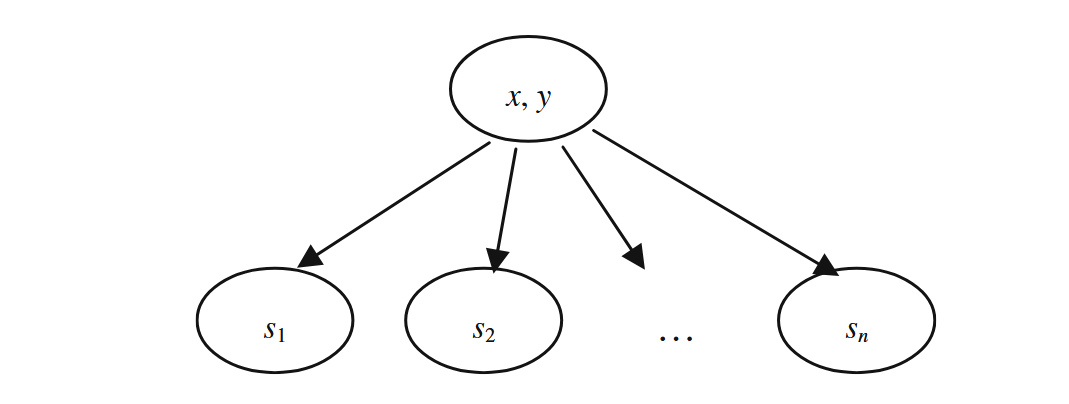
\includegraphics[width=0.4\textwidth]{Figuras/bayesian_network.PNG}
              \legend{Fonte: \cite{rfid2009review}}
        \end{figure}

        Na \autoref{fig:bayesian} temos uma representação de uma rede bayesiana para localização estacionária, onde as coordenadas $(x,y)$ representam o nó que será localizado e o $S_i$, $i=1,...,n$ são uma série de intesidades de sinais trasmitidas ou recibidas pelos pontos de refências do sistema, como nesse sistema as probabilidade de $S_i$ são idependentes e não interferem uma na outra dizemos que há uma satisfação em relação a condição de Markov \cite{rfid2009review}.
        \par
        \citeauthor{rfid2009review} afirma que a localização do dispositvo alvo pode ser obtida atravé da fórmula recursiva 
        $P((x,y) | s_1, s_2, ..., s_n) = \alpha P(s_n | (x,y)) \times P((x,y) | s_1,s_2, ...,s_{n-1})$, nessa expressão $\alpha$ é um fator de nomalização para que a soma da probabilidade posterior, no caso a primeira parte da expressão $P((x,y) | s_1, s_2, ..., s_n)$ seja uma e $(s_n | (x,y))$ calcule a probabilidade da RSSI dada para a localização do dispositivo, é importante resaltar que essa é uma expressão para localizar alvos estáticos. 
        
    \subsection{K-Nearest-Neighbor}
    Os algoritmos de vizinhaça ou no caso de \textit{nearest-neighbor} tem uma abordagem bem simples que envolve utilizar os nó ja classificados para classificar os novos nós a partir da medida de similaridade \cite{knn-3dLAN}, de outro modo, utilizar-se dos seus vizinhos para assim obter suas coordenadas com os cálculos baseados em RSS \cite{rfid2009review}.

    \par
    algumas das metricas abordada por \citeauthor{knn-3dLAN} são:

    \begin{itemize}
    \item Distância Euclidiana 
      \par
      $Dist(r,s) =  \sqrt{(x_r - x_s)(x_r - x_s)^\prime}$
    \item Padronização da Distância Euclidiana
      \par 
      $Dist(r,s) =  \sqrt{(x_r - x_s)D^-1(x_r - x_s)^\prime}$
    \item Distância de Mahalanobis
      \par
        $Dist(r,s) =  \sqrt{(x_r - x_s)V^-1(x_r - x_s)^\prime}$
    \item Distância de Manhattan
      \par
      $Dist(r,s) = \sum_{j=1}^{n} |x_{rj} - x_{sj}|$
    \item Distancia de Minkowski
      \par
      $Dist(r,s) = \sqrt[p]{\sum_{j=1}^{n}|x_{rj} - x_{sj}|^p}$

    \end{itemize}
   \par
   \citeauthor{rfid2009review} faz mostra uma outra abordagem para calcular as coordenadas do alvo obtidos a partir do sistema a seguir:
   
   $\left \{ \begin{array}{c}
        x= \sum_{i=1}^{k}w_{i}x_{i}   \\
        y= \sum_{i=1}^{k}w_{i}y_{i}  
   \end{array} \right.$ \\
    nesse sistema o $k$ representa a quantidade de vizinhos, $(x_i,y_i)$ são as coordenadas dos pontos de refências vizinhos e $w_i$ os pesos desses pontos,o cálculo dos pesos é feito a partir da diferençã de RSSI entre os pontos de refências e o alvo e as fórmulas para tal são:
    \begin{itemize}
        \item $w_i = \frac{1 / \sum_{j=1}^{m}|s_{ij} - s_{j}|}{\sum_{j=1}^{k} (1/ \sum_{j=1}^{m}|s_{ij} - s_{j}|)}$ 
        
        \item  $w_i = \frac{1 / \sqrt{\sum_{j=1}^{m}(s_{ij} - s_{j})^2}}{\sum_{j=1}^{k} (1/ \sqrt{\sum_{j=1}^{m}(s_{ij} - s_{j})^2})}$ 
    \end{itemize}$\\$
    nas expressões de $w_i$, dizemos que $s_j$ e $s_{ij}$, $j =1, ..., m$ represetam  RSSI dos respectivos ponto de referências e nó alvo que será localizado. 
    
    \subsection{Proximidade}
    A técnica de Proximidade, segundo \citeauthor{rfidProximity} baseia-se no princípio de que se o alvo está no alcance de uma antena ou leitor, sua localização será a mesma que a da antena e se o alvo está no alcance de duas ou mais antenas, a localização dada é aquela cujo possui a intensidade do sinal mais forte. Já para \citeauthor{rfid2009review} quando o alvo esta no alcance de dois ou mais receptores, utiliza-se o calculo de centroíde para estimar a localização.
    
    %\subsection{Aprendizado Baseada em Kernel}
\section{Modelagem de Sistemas}
    \subsection{UML - \textit{Unified Modeling Language}}
    O UML(em português Linguagem de Modelagem Unificada ) é uma linguagem cujo principal papel é a construção, visualização e documentação de projetos de sistemas. Surgiu na década de 90, tendo em vista que havia a necessidade de uma linguagem para modelagem que funcionasse como uma norma e fosse aceita e utilizada pela indústria, ambientes acadêmicos e de investigação \cite{uml}.
    \par
    Na UML é possível agrupar elementos e relaciona-los de maneira lógica ou estrutural, isso é o conceito de diagramas. Os elementos tem um papel importante nos modelos, eles estarão organizados de acordos com a função desempenhada no sistema, podendo representar componetes do sistema, usuário, interfaces \cite{uml}.
    
    \begin{figure}[H]
              \caption{\label{fig:uml-elementos}{Elementos UML}}
              \centering
              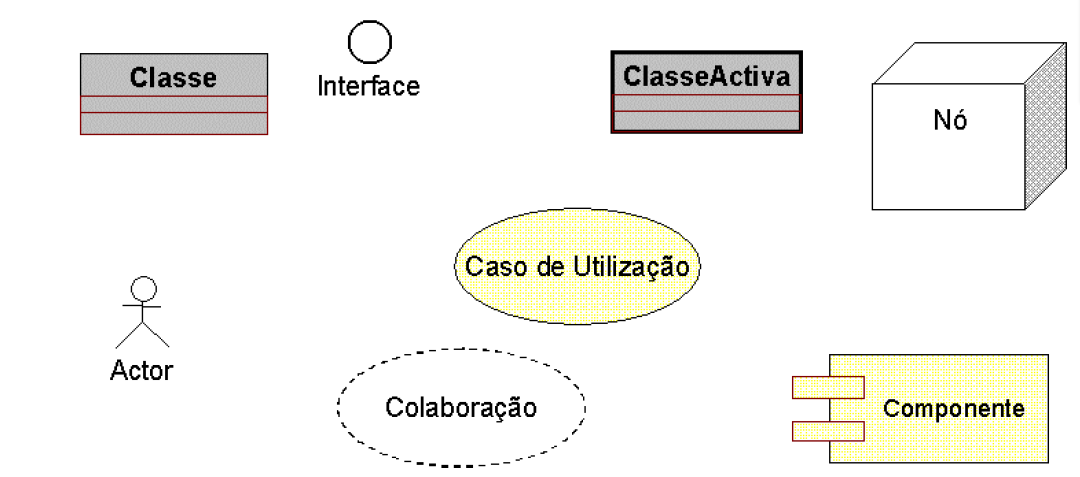
\includegraphics[width=0.9\textwidth]{Figuras/uml1.PNG}
              \legend{Fonte: \cite{uml}}
        \end{figure}
    \par
    Na \autoref{fig:uml-elementos} está um resumo de alguns elementos básicos que é utilizados em modelos de projetos de software, esses compontes por mais que sejam básicos, possibilitam a representação de vários componentes em um projeto. A seguir uma breve descrição dos diagramas comuns da UML.
    
    \begin{itemize}
       \item \textbf{Diagrama de Classe -} 
       Descreve a estrutura do sistema, como o modelo geral de informações utilizando orientação a objetos \cite{nunesfundamental}.
        
        \item \textbf{Diagrama de Caso de Uso -} 
        Descreve as funcionalidades do sistema, ou seja nesse diagrama é apresentado o'que o sistema deve fazer e os serviços que serão disponibilizados para os utilizados \cite{nunesfundamental}.
        
        \item \textbf{Diagrama de Estados -} 
        Descreve o comportamento dos objetos, as representação dos possíveis estados de um objeto e eventos que alteram valores de atributos dos objetos desencadeando as transições \cite{uml}.
        
        \item \textbf{Diagrama de Sequência -} 
        Descreve as interações dos objetos no sistema em determinado período de tempo. Essa interação é realizada por meio de troca de mensagens síncrona ou assíncrona e cada objeto possui uma linha temporal \cite{uml}.
        
        \item \textbf{Diagrama de Componentes -}
        Descreve interações entre objetos dando ênfase maior as ligações entre objetos e númerando as mensagens dessa forma não apresenta o tempo como no diagrama de sequência \cite{uml}.
        
        \item \textbf{Diagrama de Caso de Uso -} 
        Descreve as funcionalidades do sistema, ou seja nesse diagrama é apresentado o'que o sistema deve fazer e os serviços que serão disponibilizados para os utilizados \cite{nunesfundamental}.
        
        \item \textbf{Diagrama de Estados -} 
        Descreve o comportamento dos objetos, as representação dos possíveis estados de um objeto e eventos que alteram valores de atributos dos objetos desencadeando as transições \cite{uml}.
        
        \item \textbf{Diagrama de Atividade -} 
        Descreve o fluxo de trabalho que classifica os estados de "estados de atividades", onde e realizados a transições quando há a conclusão das atividades dos estados anteriores \cite{uml}.
        
        \item \textbf{Diagrama de Sequência -} 
        Descreve as interações dos objetos no sistema em determinado período de tempo. Essa interação é realizada por meio de troca de mensagens síncrona ou assíncrona e cada objeto possui uma linha temporal \cite{uml}.
        
        \item \textbf{Diagrama de Componentes -} 
        Descreve interações entre objetos dando ênfase maior as ligações entre objetos e numerando as mensagens dessa forma não apresenta o tempo como no diagrama de sequência \cite{uml}.

    \end{itemize}
    \par
 
    \subsection{Redes de Petri}